\chapter{Integrated power supply network}\label{sec:power}

Integration of the power distribution functionality with the communication infrastructure
removes the need for a dedicated power distribution network,
which has the potential to simplify the system design and reduce the complexity and weight of the wiring harnesses.
Redundant power supply topologies can be easily implemented on top of a redundant communication infrastructure.

Designs that integrate power distribution with the communication infrastructure should follow the
conventions set out in this section.

\section{Power input}

A node that draws power from the power supply network should protect its power inputs
with an over-current protection circuitry that is capable of disconnecting the input
if the power consumption of the node exceeds its design limits.
This measure is necessary to prevent a short-circuit or a similar failure of an individual node from affecting
other nodes connected to the same power supply network.

In the case of redundant power supply connections where a node is connected to more than one power supply network
concurrently, each such connection should be equipped with a circuit that prevents reverse current flow
from the node into the power supply network.
This measure is necessary to prevent a short-circuit or a similar failure of an individual power supply network
from affecting other power supply networks in the same redundant group.

\begin{figure}[H]
    \centering
    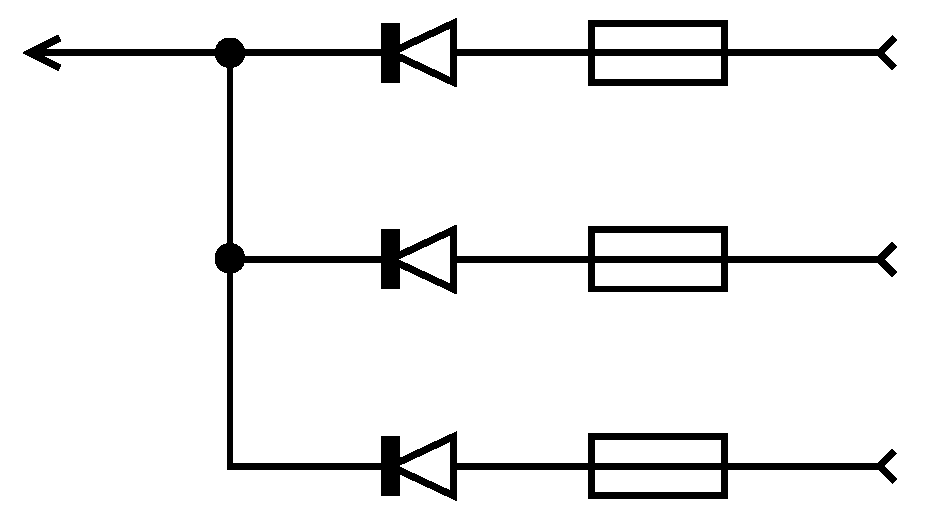
\includegraphics[width=0.3\textwidth]{redundant_power_sink}
    \caption{Redundant power input schematic}
\end{figure}

\section{Power output}

A node that delivers power to the power supply network should equip each of its power outputs
with a circuit that prevents reverse current flow from the power supply network into the node.
This measure is necessary to prevent a short-circuit or a similar failure of the node from affecting
the power supply network.

In the case of redundant power output connections where a node provides power to more than one power supply network
concurrently, each such connection should be equipped with a circuit that is capable of disconnecting the output
if the power consumption per network exceeds the design limits.
This measure is necessary to prevent a short-circuit or a similar failure of an individual power supply network
from affecting other power supply networks in the same redundant group.

\begin{figure}[H]
    \centering
    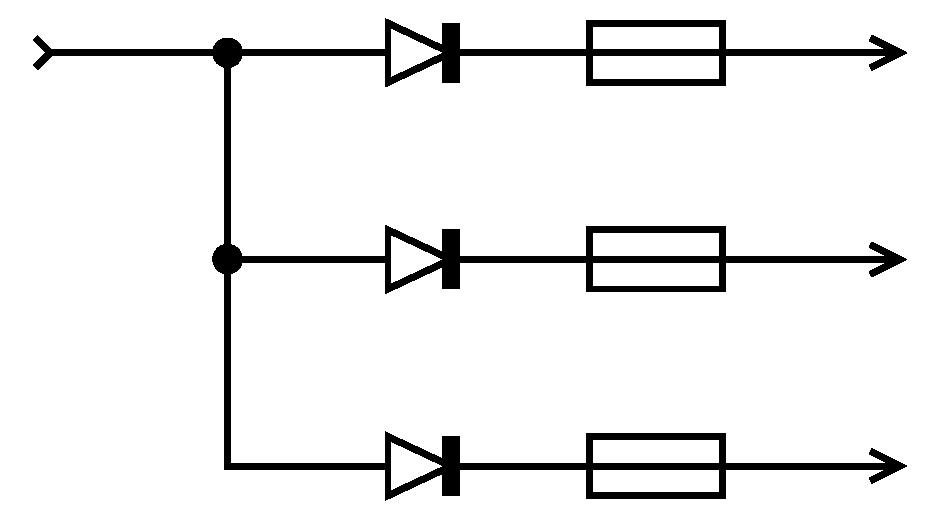
\includegraphics[width=0.3\textwidth]{redundant_power_source}
    \caption{Redundant power output schematic}
\end{figure}
